\documentclass{mylabreport}
\usepackage{pifont}

\graphicspath{{./figures/}, {./figures/outputs/}}


\setlabnumber{01} 
\setcoursecode{CSE 4733} 
\setcoursetitle{Digital Image Processing} 
\setlabtitle{Canny Edge Detector} 
\setstudentid{200041225} 
\setstudent{ 
    \textbf{K. M. Abesh Ahsan} \\
    200041225 \\
    Section 2 \\
} 

% -------------------------------------------------
%
%
% Start of the document
% -------------------------------------------------

\begin{document}

\maketitlepage
\customtableofcontents
\newpage

\section{Introduction}
\label{sec:introduction}

The \textbf{Canny edge detector} is an \href{https://en.wikipedia.org/wiki/Edge_detection}{edge detection} operator that uses a multi-stage algorithm to detect a wide range of edges in images. It was developed by \href{https://en.wikipedia.org/wiki/John_F._Canny}{John F. Canny} in 1986. He also produced a computational theory of edge detection explaining why the technique works \cite{wikipedia_canny}.

In this report, the Canny edge detection algorithm has been implemented using the resources and explanations provided in \cite{gonzalez2008, medium_canny, sriram_canny, wikipedia_canny}. 

My implementation is available at: \url{https://github.com/abeshahsan/Assignment---Canny-Edge-Detector}

\subsection{Why Canny?}
\label{sec:why-canny}
The Canny edge detector was developed to address key limitations of simpler methods like the Sobel filter, which only computes gradient magnitude and direction. The motivation stemmed from three main goals:

Noise Reduction: Sobel is sensitive to noise, as it directly computes gradients without smoothing.

Edge Thinning: Sobel produces thick edges, while Canny uses non-maximum suppression to yield single-pixel-wide edges.

Edge Connectivity: Sobel relies on a single threshold, often creating fragmented edges. Canny employs hysteresis thresholding (dual thresholds) to link weak edges to strong ones, improving continuity.

\subsection{Why Canny over Sobel?}
\label{sec:why-canny-over-sobel}

Sobel alone lacks noise suppression, generates thick edges, and struggles with false positives/negatives due to basic thresholding. Canny integrates Gaussian smoothing, edge thinning, and intelligent thresholding, making it more robust, precise, and reliable for real-world applications where edge quality is critical.


\subsection{Canny Edge Detection Algorithm}
\label{sec:canny-edge-detection-algorithm}
The Canny edge detection algorithm is a multi-step process that involves several stages to ensure accurate and reliable edge detection. The main steps of the Canny edge detection algorithm are as follows:
\begin{enumerate}
    \item Noise Reduction
    \item Gradient Calculation
    \item Non-maximum Suppression
    \item Double Threshold
    \item Edge Tracking by Hysteresis
\end{enumerate}

In the subsequent sections, we will delve into each of these steps in detail.

To illustrate the Canny edge detection algorithm, we will use the image shown in \autoref{fig:lena-original} as an example. The result of applying the algorithm is depicted in \autoref{fig:lena-edge}.

\begin{figure}[ht]
    \centering
    \begin{subfigure}[b]{0.4\textwidth}
        \centering
        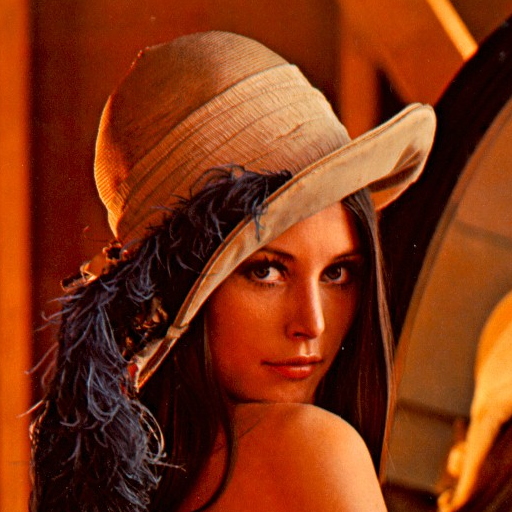
\includegraphics[width=0.9\textwidth]{lenna_1_original.png}
        \caption{Original Image}
        \label{fig:lena-original}
    \end{subfigure}
    \hfill
    \begin{subfigure}[b]{0.4\textwidth}
        \centering
        
\includegraphics[width=0.9\textwidth]{lenna_8_canny_edge_detected.png}
        \caption{Edge Detected Image}
        \label{fig:lena-edge}
    \end{subfigure}
    \caption{Comparison of Original and Edge Detected Images using Canny Edge Detection Algorithm}
    \label{fig:lena-comparison}
\end{figure}


\section{Grayscale Conversion}
\label{sec:grayscale-conversion}

The Canny Edge Detection algorithm operates on grayscale images. This is because edge detection is primarily concerned with changes in intensity. Converting a color image to grayscale simplifies the computation and focuses on the luminance information, which is crucial for detecting edges.

The effect after converting a color image to grayscale is shown in \autoref{fig:color-vs-grayscale}.

\begin{figure}[ht]
    \centering
    \begin{subfigure}[b]{0.4\textwidth}
        \centering
        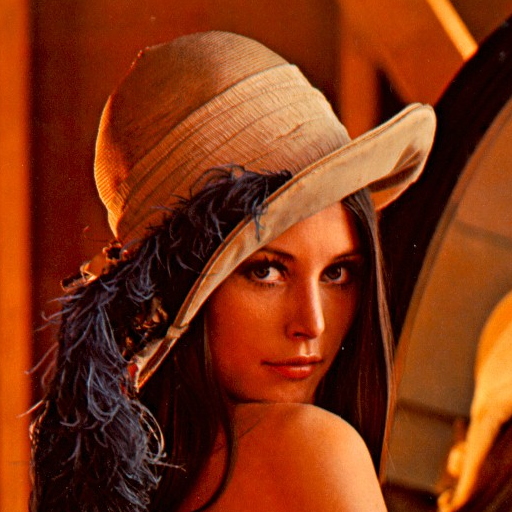
\includegraphics[width=0.9\textwidth]{lenna_1_original.png}
        \caption{Original Color Image}
        \label{fig:lena-color}
    \end{subfigure}
    \hfill
    \begin{subfigure}[b]{0.4\textwidth}
        \centering
        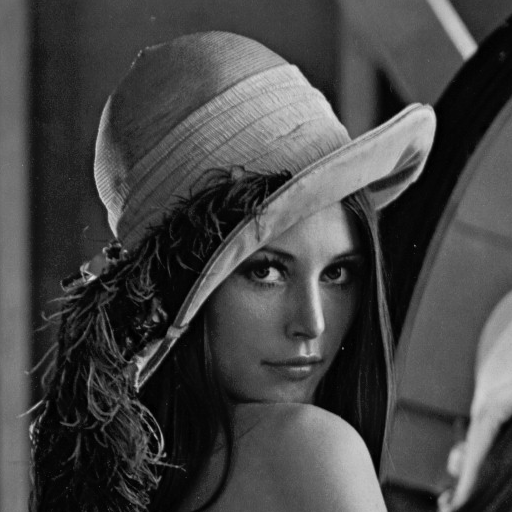
\includegraphics[width=0.9\textwidth]{lenna_2_grayscale.png}
        \caption{Grayscale Image}
        \label{fig:lena-grayscale}
    \end{subfigure}
    \caption{Output of Converting a Color Image to Grayscale}
    \label{fig:color-vs-grayscale}
\end{figure}
\section{Noise Reduction}
\label{sec:noise-reduction}

The method of \emph{Canny edge detection} is solely based on gradients, and the gradient calculation is very sensitive to noise. So, it is necessary to reduce noise in the image before applying the edge detection algorithm. There are several methods to reduce noise in an image. The most common method is to apply a \emph{Gaussian filter} to the image. It is a low-pass filter that removes high-frequency noise from the image; i.e., it smoothens the image.

\begin{equation}
    \label{eq:gaussian-filter}
    H(x, y) = \frac{1}{2\pi\sigma^2}e^{-\frac{x^2 + y^2}{2\sigma^2}}
\end{equation}

Where, $H(x, y)$ is the Gaussian filter, $\sigma$ is the standard deviation of the Gaussian distribution, and $x$ and $y$ are the coordinates of the filter. The Gaussian filter is applied to the image using convolution.

After applying the Gaussian filter, the image becomes less noisy, and the edges become more pronounced. This is illustrated in \autoref{fig:noise-reduction}.

\begin{figure}[ht]
    \centering
    \begin{subfigure}[b]{0.4\textwidth}
        \centering
        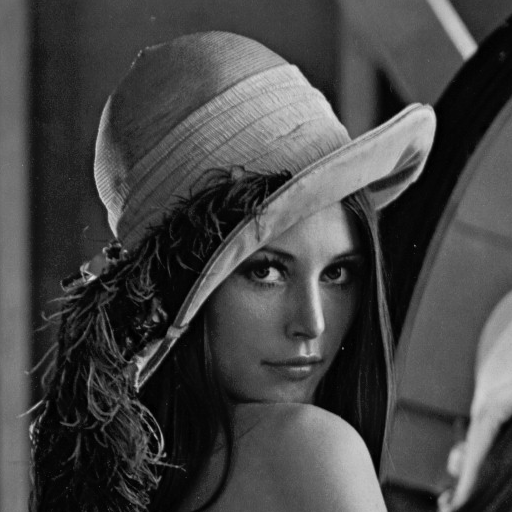
\includegraphics[width=0.9\textwidth]{lenna_2_grayscale.png}
        \caption{Original Grayscale Image}
        \label{fig:grayscale-original}
    \end{subfigure}
    \hfill
    \begin{subfigure}[b]{0.4\textwidth}
        \centering
        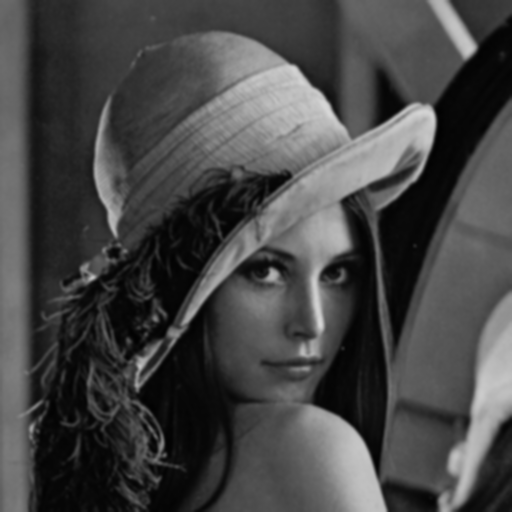
\includegraphics[width=0.9\textwidth]{lenna_3_blurred.png}
        \caption{Image after Applying Gaussian Filter ($5\times5$)}
        \label{fig:gaussian-filter}
    \end{subfigure}
    \caption{Effect of Noise Reduction on an Image}
    \label{fig:noise-reduction}
\end{figure}
\section{Edge Detection}
\label{sec:edge-detection}

Edge detection is a fundamental task in image processing and computer vision, aimed at identifying points in an image where the intensity changes sharply. These points typically correspond to object boundaries and other significant features within the image.

The gradient of an image is a vector that has both magnitude and direction. The magnitude indicates the strength of the edge, while the direction indicates the orientation of the edge (to be more precise, the shape of the object).

\subsection{Sobel Operator}
\label{subsec:sobel-operator}

The \emph{Sobel operator} is a widely used edge detection technique that employs two convolution kernels to estimate the gradient of the image intensity. One kernel is used to calculate the gradient in the x-direction, while the other is used to calculate the gradient in the y-direction.

\paragraph{Sobel Operator in the x-direction}
The convolution kernel for the \emph{Sobel} operator in the x-direction is defined as:
\begin{equation}
    G_x =
    \begin{bmatrix}
        -1 & 0 & 1 \\
        -2 & 0 & 2 \\
        -1 & 0 & 1
    \end{bmatrix}
    \label{eq:sobel_x}
\end{equation}

\paragraph{Sobel Operator in the y-direction}
The convolution kernel for the \emph{Sobel} operator in the y-direction is defined as:
\begin{equation}
    G_y =
    \begin{bmatrix}
        -1 & -2 & -1 \\
        0  & 0  & 0  \\
        1  & 2  & 1
    \end{bmatrix}
    \label{eq:sobel_y}
\end{equation}

\subsection{Magnitude and Direction of the Gradient}
\label{subsec:magnitude-and-direction}

The gradient magnitude and direction are essential for understanding the strength and orientation of edges in an image. These can be computed using the gradients in the x and y directions, \( G_x \) and \( G_y \), respectively.

\paragraph{Gradient Magnitude}
The magnitude of the gradient can be calculated using two different norms:

\begin{itemize}
    \item \textbf{L1 Norm:}
          \begin{equation}
              \text{Magnitude}_{L1} = |G_x| + |G_y|
              \label{eq:grad-magnitude-l1}
          \end{equation}
    \item \textbf{L2 Norm:}
          \begin{equation}
              \text{Magnitude}_{L2} = \sqrt{G_x^2 + G_y^2}
              \label{eq:grad-magnitude-l2}
          \end{equation}
\end{itemize}

\paragraph{Gradient Direction}
The direction of the gradient indicates the orientation of the edge and is computed as follows:
\begin{equation}
    \text{Direction} = \arctan\left(\frac{G_y}{G_x}\right)
    \label{eq:grad-direction}
\end{equation}

The gradient direction is typically measured in radians and can be converted to degrees if needed.

The result of applying the Sobel operator to an image is shown in \autoref{fig:sobel-gradient}.

\begin{figure}[ht]
    \centering
    \begin{subfigure}[b]{0.4\textwidth}
        \centering
        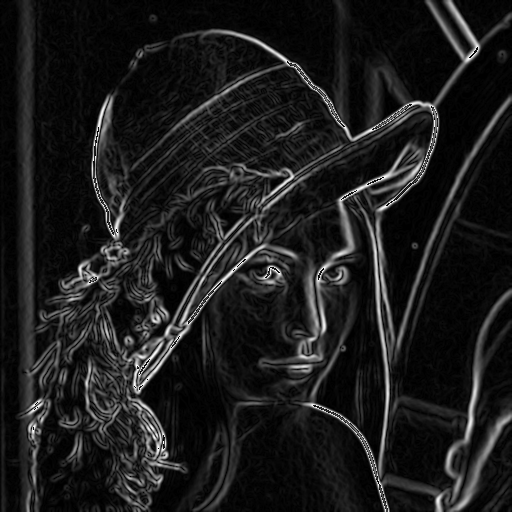
\includegraphics[width=0.9\textwidth]{lenna_4_gradient_magnitude.png}
        \caption{Gradient Magnitude}
        \label{fig:gradient-magnitude}
    \end{subfigure}
    \hfill
    \begin{subfigure}[b]{0.4\textwidth}
        \centering
        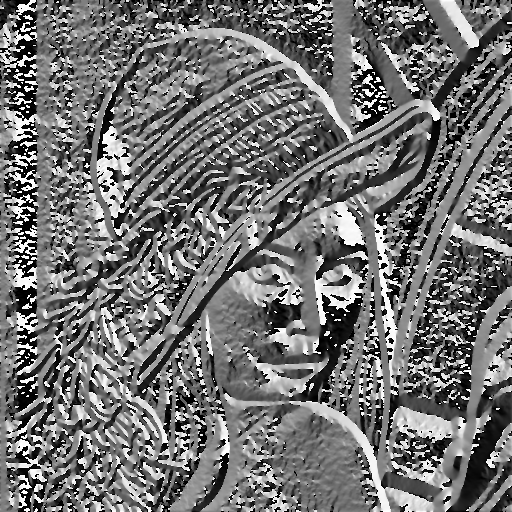
\includegraphics[width=0.9\textwidth]{lenna_5_gradient_direction.png}
        \caption{Gradient Direction}
        \label{fig:gradient-direction}
    \end{subfigure}
    \caption{Gradient Magnitude and Direction using Sobel Operator}
    \label{fig:sobel-gradient}
\end{figure}


It is important to note in \autoref{fig:gradient-direction} that the gradient direction can have both positive and negative values. Consequently, when visualizing the image, negative values are automatically truncated.
\section{Non-Maximum Suppression}

Non-Maximum Suppression (NMS) is a technique used to thin out the edges detected in the gradient image, ensuring that only the most significant edges are retained. This step is essential for refining the edge map and removing spurious responses, which helps in accurately identifying the true edges in an image.

Technically, NMS examines the gradient magnitude and direction at each pixel, comparing it with neighboring pixels along the gradient direction. If the current pixel's magnitude is not the maximum, it is suppressed (set to zero); otherwise, it is retained. This ensures that only local maxima are preserved, resulting in a thinned edge map.

In simpler terms, NMS sharpens blurry, thick edges by keeping only the highest points along an edge direction, like tracing an outline with a fine-tipped pen instead of a broad marker.

The process of Non-Maximum Suppression can be broken down into the following steps:

\begin{enumerate}
    \item Compute the gradient direction for each pixel in the gradient image using \autoref{eq:grad-direction}.
    \item For each pixel, compare its gradient magnitude with the magnitudes of the two neighboring pixels along the gradient direction.
    \item If the pixel's magnitude is not the maximum among the three, set it to zero; otherwise, retain its value.
\end{enumerate}


See in \autoref{fig:nms-examples} for an example of how NMS works. The cell enclosed by red-dashed border is the current pixel that is being processed. The two neighboring pixels with black-dashed borders are the pixels that falls in the gradient direction of the current pixel. In \autoref{fig:nms1} the current pixel's gradient direction is $pi$. And in \autoref{fig:nms2} the current pixel's gradient direction is $5pi/4$.
\autoref{fig:nms1} shows the case when the current pixel is a local maximum. In this case, the current pixel is retained. So, no suppression is done. \autoref{fig:nms2} shows the case when the current pixel is not a local maximum. In this case, the current pixel is suppressed. So, the pixel is set to zero.

\begin{figure}
    \centering
    \begin{subfigure}[b]{0.40\textwidth}
        \centering
        \begin{subfigure}[b]{0.40\textwidth}
            \renewcommand\thesubfigure{\alph{subfigure}1}
            \centering
            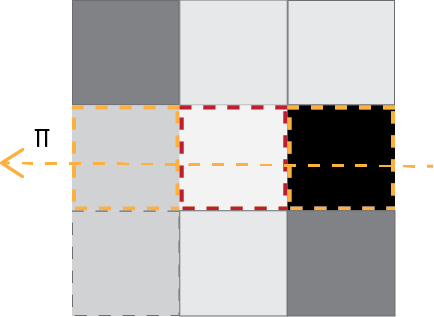
\includegraphics[width=0.9\textwidth]{nms1-before.png}
            \caption{Before NMS}
            \label{fig:nms1-before}
        \end{subfigure}
        \hfill
        \begin{subfigure}[b]{0.40\textwidth}
            \addtocounter{subfigure}{-1}
            \renewcommand\thesubfigure{\alph{subfigure}2}
            \centering
            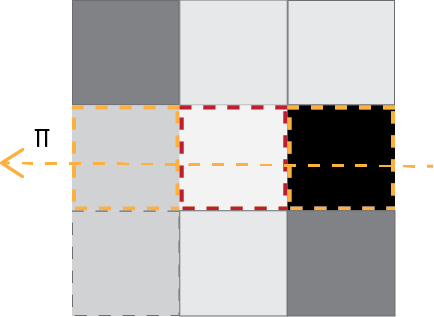
\includegraphics[width=0.9\textwidth]{nms1-after.png}
            \caption{After NMS}
            \label{fig:nms1-after}
        \end{subfigure}

        \addtocounter{subfigure}{-1}
        \caption{No Suppression}
        \label{fig:nms1}

    \end{subfigure}
    \hfill

    \vspace{0.75cm}

    \begin{subfigure}[b]{0.40\textwidth}
        \centering
        \begin{subfigure}[b]{0.40\textwidth}
            \renewcommand\thesubfigure{\alph{subfigure}1}
            \centering
            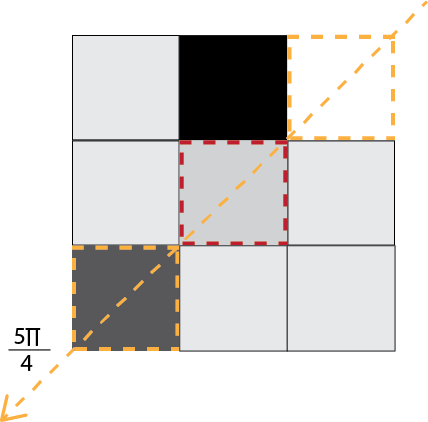
\includegraphics[width=0.9\textwidth]{nms2-before.png}
            \caption{Before NMS}
            \label{fig:nms2-before}
        \end{subfigure}
        \hfill
        \begin{subfigure}[b]{0.40\textwidth}
            \addtocounter{subfigure}{-1}
            \renewcommand\thesubfigure{\alph{subfigure}2}
            \centering
            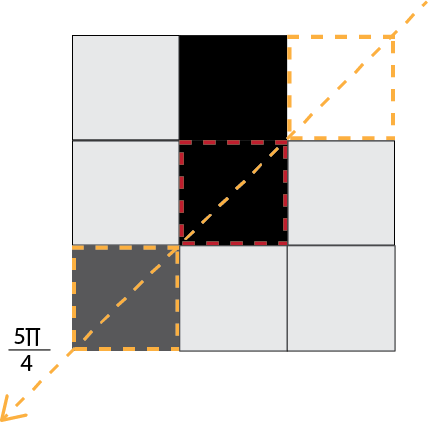
\includegraphics[width=0.9\textwidth]{nms2-after.png}
            \caption{After NMS}
            \label{fig:nms2-after}
        \end{subfigure}
        \addtocounter{subfigure}{-1}
        \caption{Suppression}
        \label{fig:nms2}
    \end{subfigure}
    \caption{Visualization of Non-Maximum Suppression}
    \label{fig:nms-examples}
\end{figure}

The result of applying non-maximum suppression to the gradient magnitude image is shown in \autoref{fig:nms}.

\begin{figure}[ht]
    \centering
    \begin{subfigure}[b]{0.4\textwidth}
        \centering
        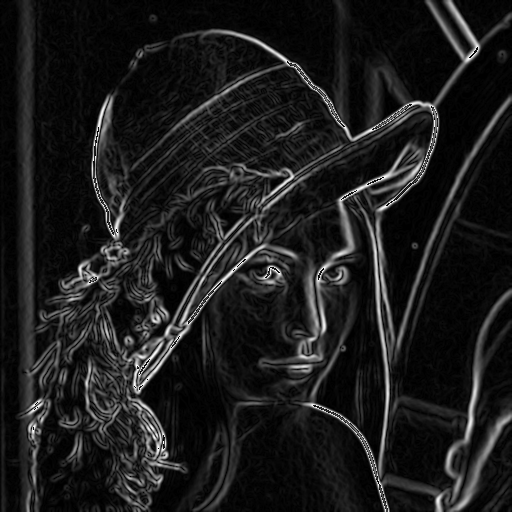
\includegraphics[width=0.9\textwidth]{lenna_4_gradient_magnitude.png}
        \caption{Gradient Magnitude}
        \label{fig:gradient-magnitude-wo-nms}
    \end{subfigure}
    \hfill
    \begin{subfigure}[b]{0.4\textwidth}
        \centering
        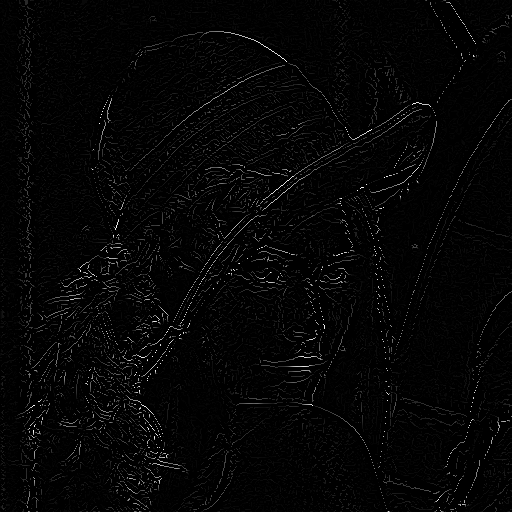
\includegraphics[width=0.9\textwidth]{lenna_6_non_max_suppressed.png}
        \caption{After Non-Maximum Suppression}
        \label{fig:gradient-magnitude-with-nms}
    \end{subfigure}
    \caption{Effect of Non-Maximum Suppression on Gradient Magnitude}
    \label{fig:nms}
\end{figure}
\section{Double Thresholding}
\label{sec:double-thresholding}

Following non-maximum suppression, the edge pixels provide a clearer representation of true edges in the image. Nonetheless, some edge pixels might still appear due to noise and color differences. To eliminate these false positives, it is essential to discard edge pixels with low gradient values while retaining those with high gradient values.

This is achieved through a process called \emph{double thresholding}.

The Canny edge detector uses double thresholding to classify edge pixels into three categories: strong edges, weak edges, and non-edge pixels. The process is as follows:

\begin{enumerate}
    \item \textbf{Strong Edges:} Pixels with gradient magnitudes higher than a high threshold are classified as strong edges.
    \item \textbf{Non-Edge Pixels:} Pixels with gradient magnitudes lower than a low threshold are classified as non-edge pixels.
    \item \textbf{Weak Edges:} Pixels with gradient magnitudes between the high and low thresholds are classified as weak edges.
\end{enumerate}

The high and low thresholds are determined based on the gradient magnitude distribution in the image. Typically, the high threshold is set to a value that retains only strong edges, while the low threshold is set to a fraction of the high threshold.

In my version of implementation, I used ratios for the threshold --- $ T_{\text{high}} $ and $ T_{\text{high}} $ --- to determine the high and low thresholds. The ratios are provided as input parameters to the function. Then the high and low thresholds are calculated as follows:

\begin{align*}
    T_{\text{high}} & = r_{\text{max}} \cdot r_{\text{high\_ratio}} \\
    T_{\text{low}}  & = T_{\text{high}} \cdot r_{\text{low\_ratio}}
\end{align*}

The \emph{strong pixels} are assigned a value of 255, the \emph{weak pixels} are assigned a value lower than 255 (e.g., 100), and the \emph{non-edge pixels} are assigned a value of 0.

The images before and after double thresholding are shown in \autoref{fig:double-thresholding}.

\begin{figure}[ht]
    \centering
    \begin{subfigure}[b]{0.4\textwidth}
        \centering
        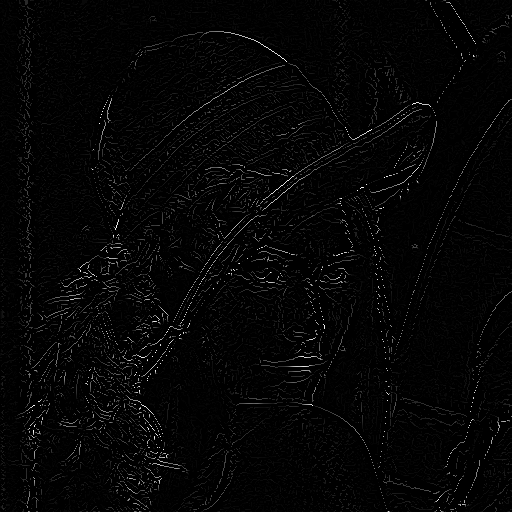
\includegraphics[width=0.9\textwidth]{lenna_6_non_max_suppressed.png}
        \caption{After Non-Maximum Suppression}
    \end{subfigure}
    \hfill
    \begin{subfigure}[b]{0.4\textwidth}
        \centering
        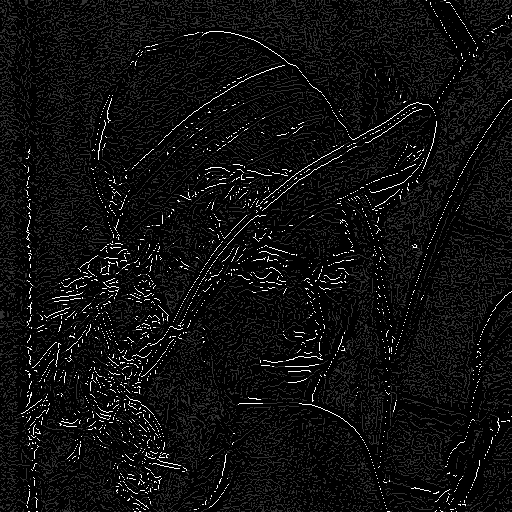
\includegraphics[width=0.9\textwidth]{lenna_7_double_thresholded.png}
        \caption{After Double Thresholding}
    \end{subfigure}
    \caption{Effect of Double Thresholding}
    \label{fig:double-thresholding}
\end{figure}
\section{Hysteresis}
\label{sec:hysteresis}

The final step in the Canny edge detection algorithm is edge linking through a process called \emph{hysteresis}. This step aims to connect weak edge pixels to strong edge pixels to form continuous and complete edges in the image.

What hysteresis does is, it helps to eliminate false edges by considering the connectivity of weak edges to strong edges. The idea is that if a weak edge pixel is connected to a strong edge pixel, it should be retained as part of the edge. Conversely, if a weak edge pixel is not connected to any strong edge pixels, it should be discarded.

The hysteresis process involves the following steps:

\begin{enumerate}
    \item Examine a weak edge pixel and its 8-connected neighborhood pixels.
    \item Identify if there is at least one strong edge pixel in the neighborhood.
    \item If a strong edge pixel is found, preserve the weak edge pixel as part of the edge, i.e., convert it to a strong edge pixel.
    \item Repeat the process for neighboring weak edge pixels to ensure continuity.
\end{enumerate}

The visualization of the hysteresis process is shown in \autoref{fig:hysteresis-example}. In the first case, the weak edge pixel has no strong edge neighbors, so it is set to 0. In the second case, the weak edge pixel has (at least one) strong edge neighbors, so it is set to 255.

\begin{figure}[ht]
    \centering
    \begin{subfigure}[b]{0.4\textwidth}
        \centering
        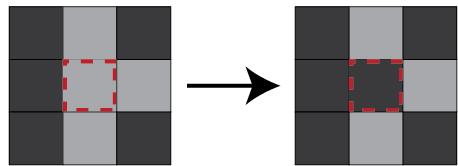
\includegraphics[width=0.9\textwidth]{hysteresis-no-strong-around.png}
        \caption{Weak Pixel with No Strong Neighbors (Set to 0)}
        \label{fig:hysteresis-no-strong-around}
    \end{subfigure}
    \hfill
    \begin{subfigure}[b]{0.4\textwidth}
        \centering
        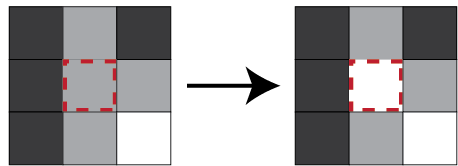
\includegraphics[width=0.9\textwidth]{hysteresis-one-strong-around.png}
        \caption{Weak Pixel with Strong Neighbors (Set to 255)}
        \label{fig:hysteresis-one-strong-around}
    \end{subfigure}
    \caption{Effect of Hysteresis on Weak Edge Pixels}
    \label{fig:hysteresis-example}
\end{figure}

The result of the hysteresis process is a binary image with strong edges that are connected to weak edges, forming complete edges in the image, as shown in \autoref{fig:hysteresis}.

\begin{figure}[ht]
    \centering
    \begin{subfigure}[b]{0.4\textwidth}
        \centering
        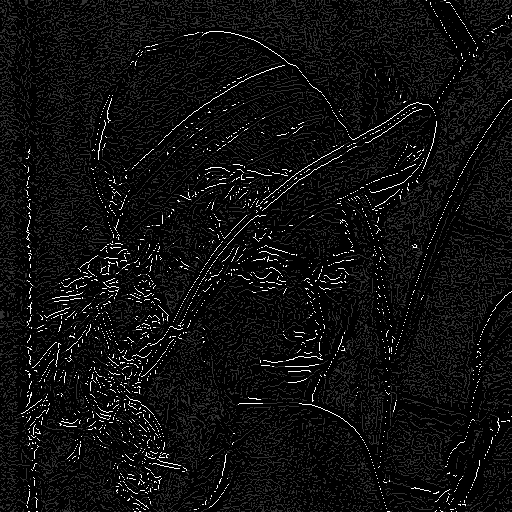
\includegraphics[width=0.9\textwidth]{lenna_7_double_thresholded.png}
        \caption{After Double Thresholding}
    \end{subfigure}
    \hfill
    \begin{subfigure}[b]{0.4\textwidth}
        \centering
        
\includegraphics[width=0.9\textwidth]{lenna_8_canny_edge_detected.png}
        \caption{After Hysteresis}
    \end{subfigure}
    \caption{Effect of Hysteresis}
    \label{fig:hysteresis}
\end{figure}

\section{Results}
\label{sec:results}

\subsection{Some Results Using Different Images}

The Canny Edge Detector was applied to various images, demonstrating its effectiveness in edge detection. The results are shown in \autoref{fig:lenna_grayscale} to \autoref{fig:car_edge_detected}. Each image is presented in grayscale and with the edges detected using the Canny method.

\begin{figure}[ht]
    \centering
    \begin{subfigure}{0.4\textwidth}
        \centering
        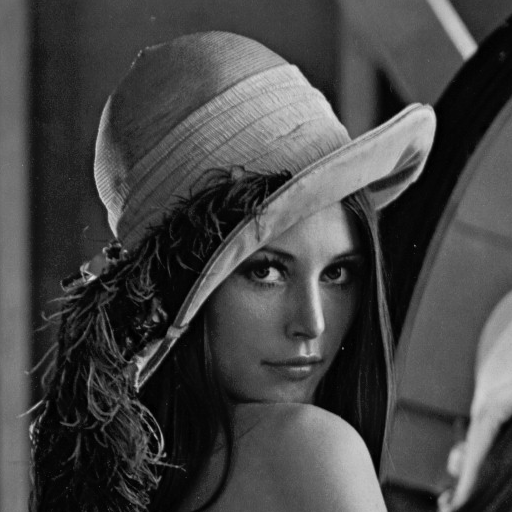
\includegraphics[width=0.9\textwidth]{lenna_2_grayscale.png}
        \caption{Lenna Grayscale}
        \label{fig:lenna_grayscale}
    \end{subfigure}
    \hfill
    \begin{subfigure}{0.4\textwidth}
        \centering
        
\includegraphics[width=0.9\textwidth]{lenna_8_canny_edge_detected.png}
        \caption{Lenna Edge Detected}
        \label{fig:lenna_edge_detected}
    \end{subfigure}
    \caption{Canny Edge Detection Results for Different Images (Part 1)}
\end{figure}

\begin{figure}[ht]\ContinuedFloat
    \centering
    \begin{subfigure}{0.4\textwidth}
        \centering
        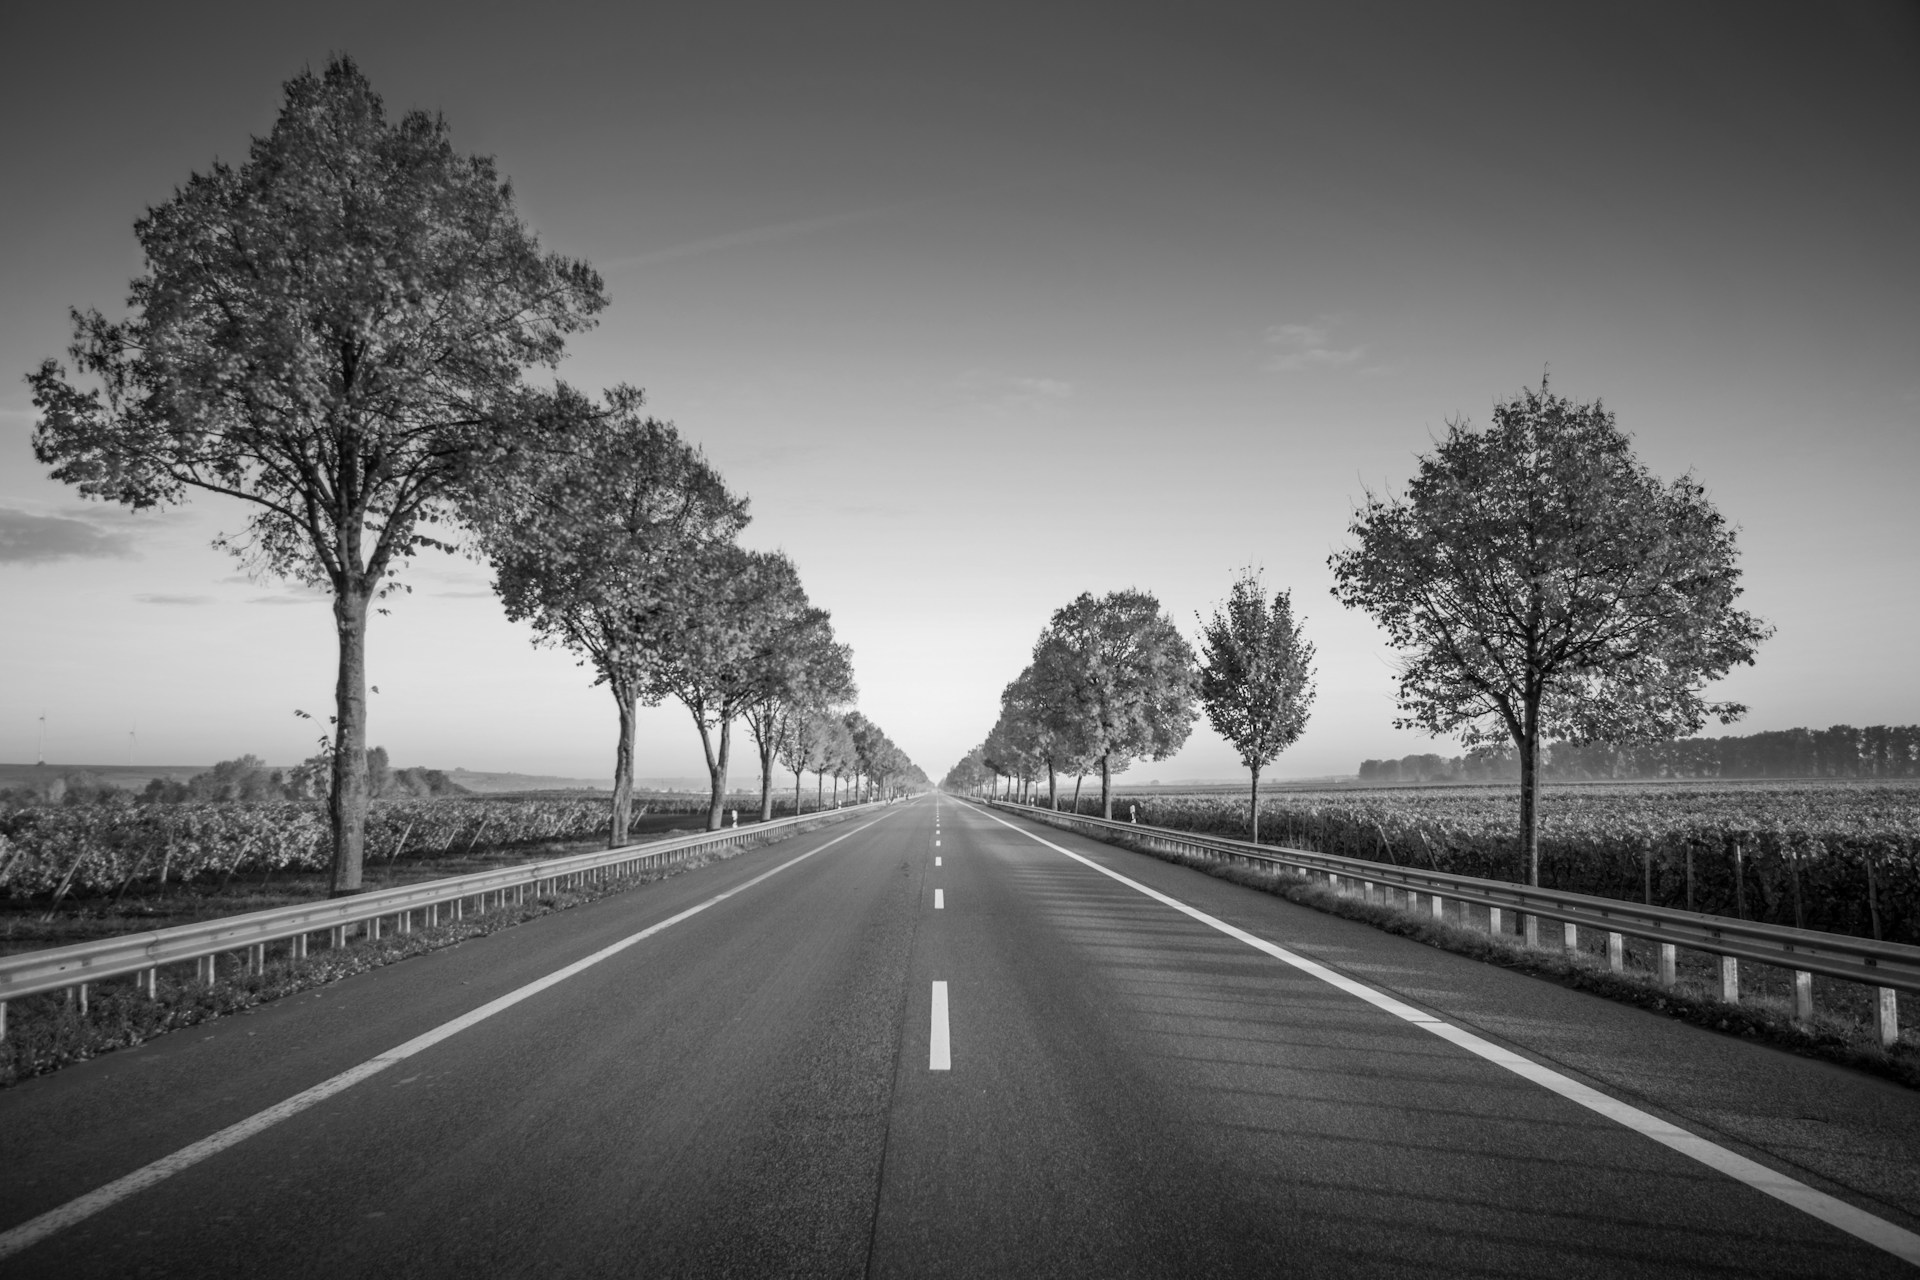
\includegraphics[width=0.9\textwidth]{road_2_grayscale.png}
        \caption{Road Grayscale}
        \label{fig:road_grayscale}
    \end{subfigure}
    % \hfill
    \begin{subfigure}{0.4\textwidth}
        \centering
        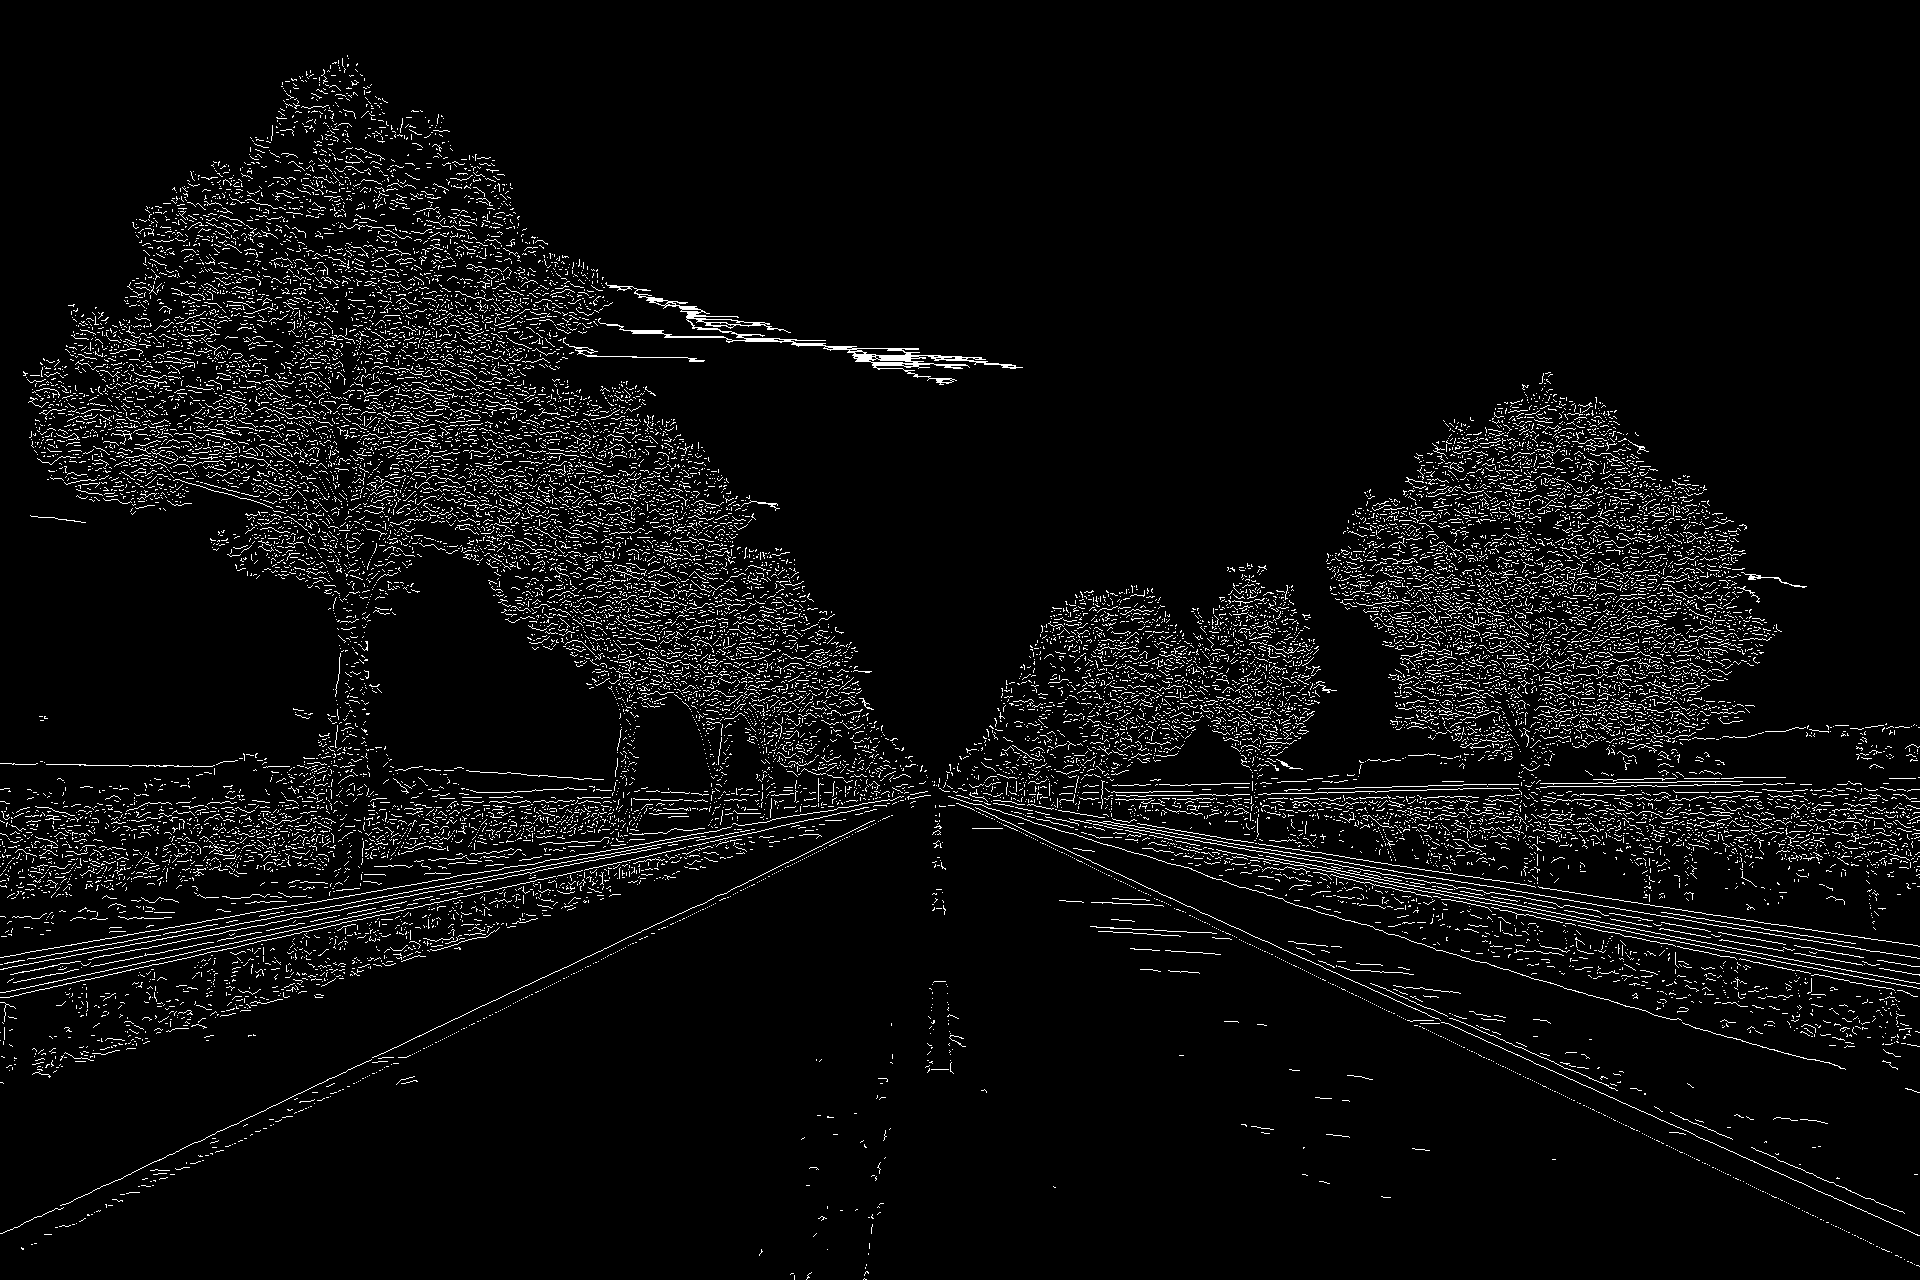
\includegraphics[width=0.9\textwidth]{road_8_canny_edge_detected.png}
        \caption{Road Edge Detected}
        \label{fig:road_edge_detected}
    \end{subfigure}
    \caption{Canny Edge Detection Results for Different Images (Part 2)}
\end{figure}

\begin{figure}[ht]\ContinuedFloat
    \centering
    \begin{subfigure}{0.4\textwidth}
        \centering
        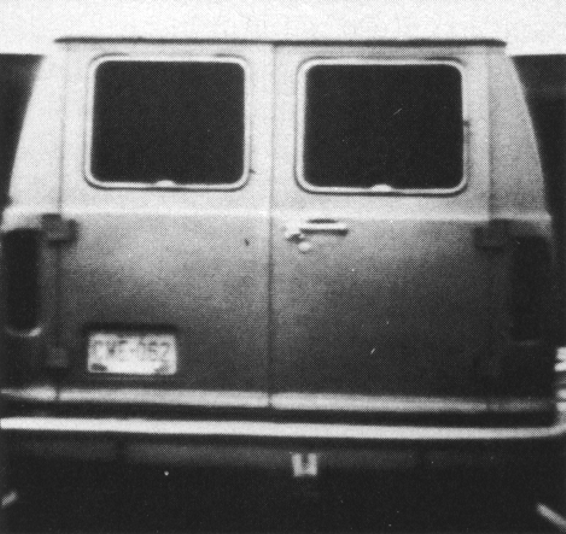
\includegraphics[width=0.9\textwidth]{van_2_grayscale.png}
        \caption{Van Grayscale}
        \label{fig:van_grayscale}
    \end{subfigure}
    % \hfill
    \begin{subfigure}{0.4\textwidth}
        \centering
        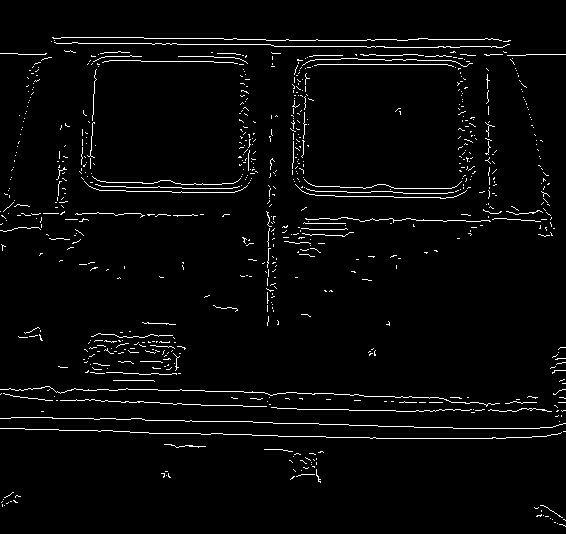
\includegraphics[width=0.9\textwidth]{van_8_canny_edge_detected.png}
        \caption{Van Edge Detected}
        \label{fig:van_edge_detected}
    \end{subfigure}
    \caption{Canny Edge Detection Results for Different Images (Part 3)}
\end{figure}

\begin{figure}[ht]\ContinuedFloat
    \centering
    \begin{subfigure}{0.4\textwidth}
        \centering
        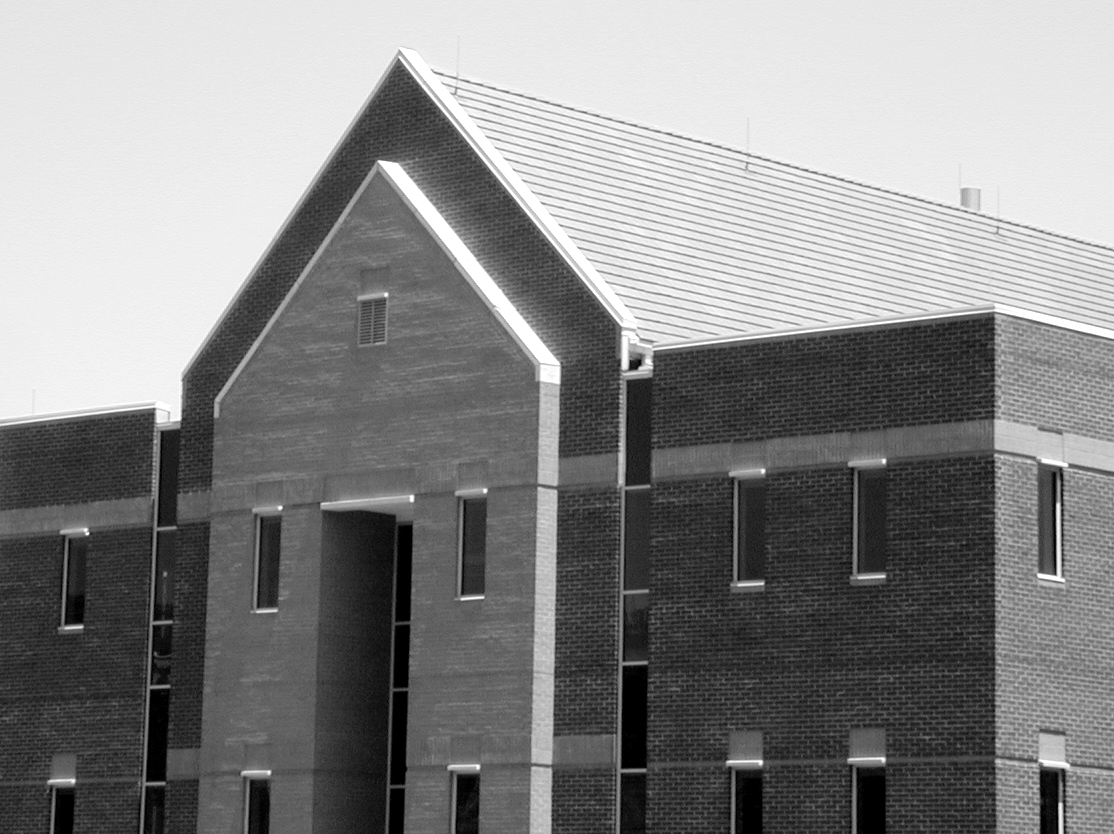
\includegraphics[width=0.9\textwidth]{building_2_grayscale.png}
        \caption{Building Grayscale}
        \label{fig:building_grayscale}
    \end{subfigure}
    \hfill
    \begin{subfigure}{0.4\textwidth}
        \centering
        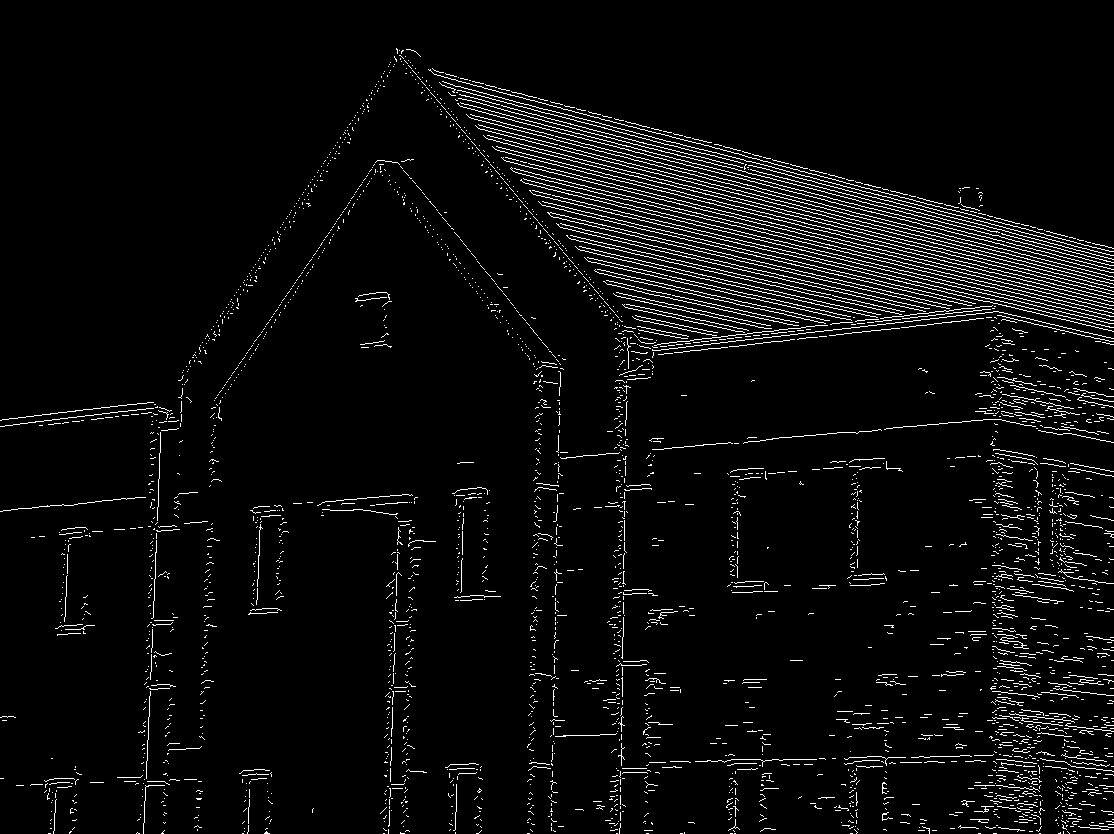
\includegraphics[width=0.9\textwidth]{building_8_canny_edge_detected.png}
        \caption{Building Edge Detected}
        \label{fig:building_edge_detected}
    \end{subfigure}
    \caption{Canny Edge Detection Results for Different Images (Part 4)}
\end{figure}

\begin{figure}[ht]\ContinuedFloat
    \centering
    \begin{subfigure}{0.4\textwidth}
        \centering
        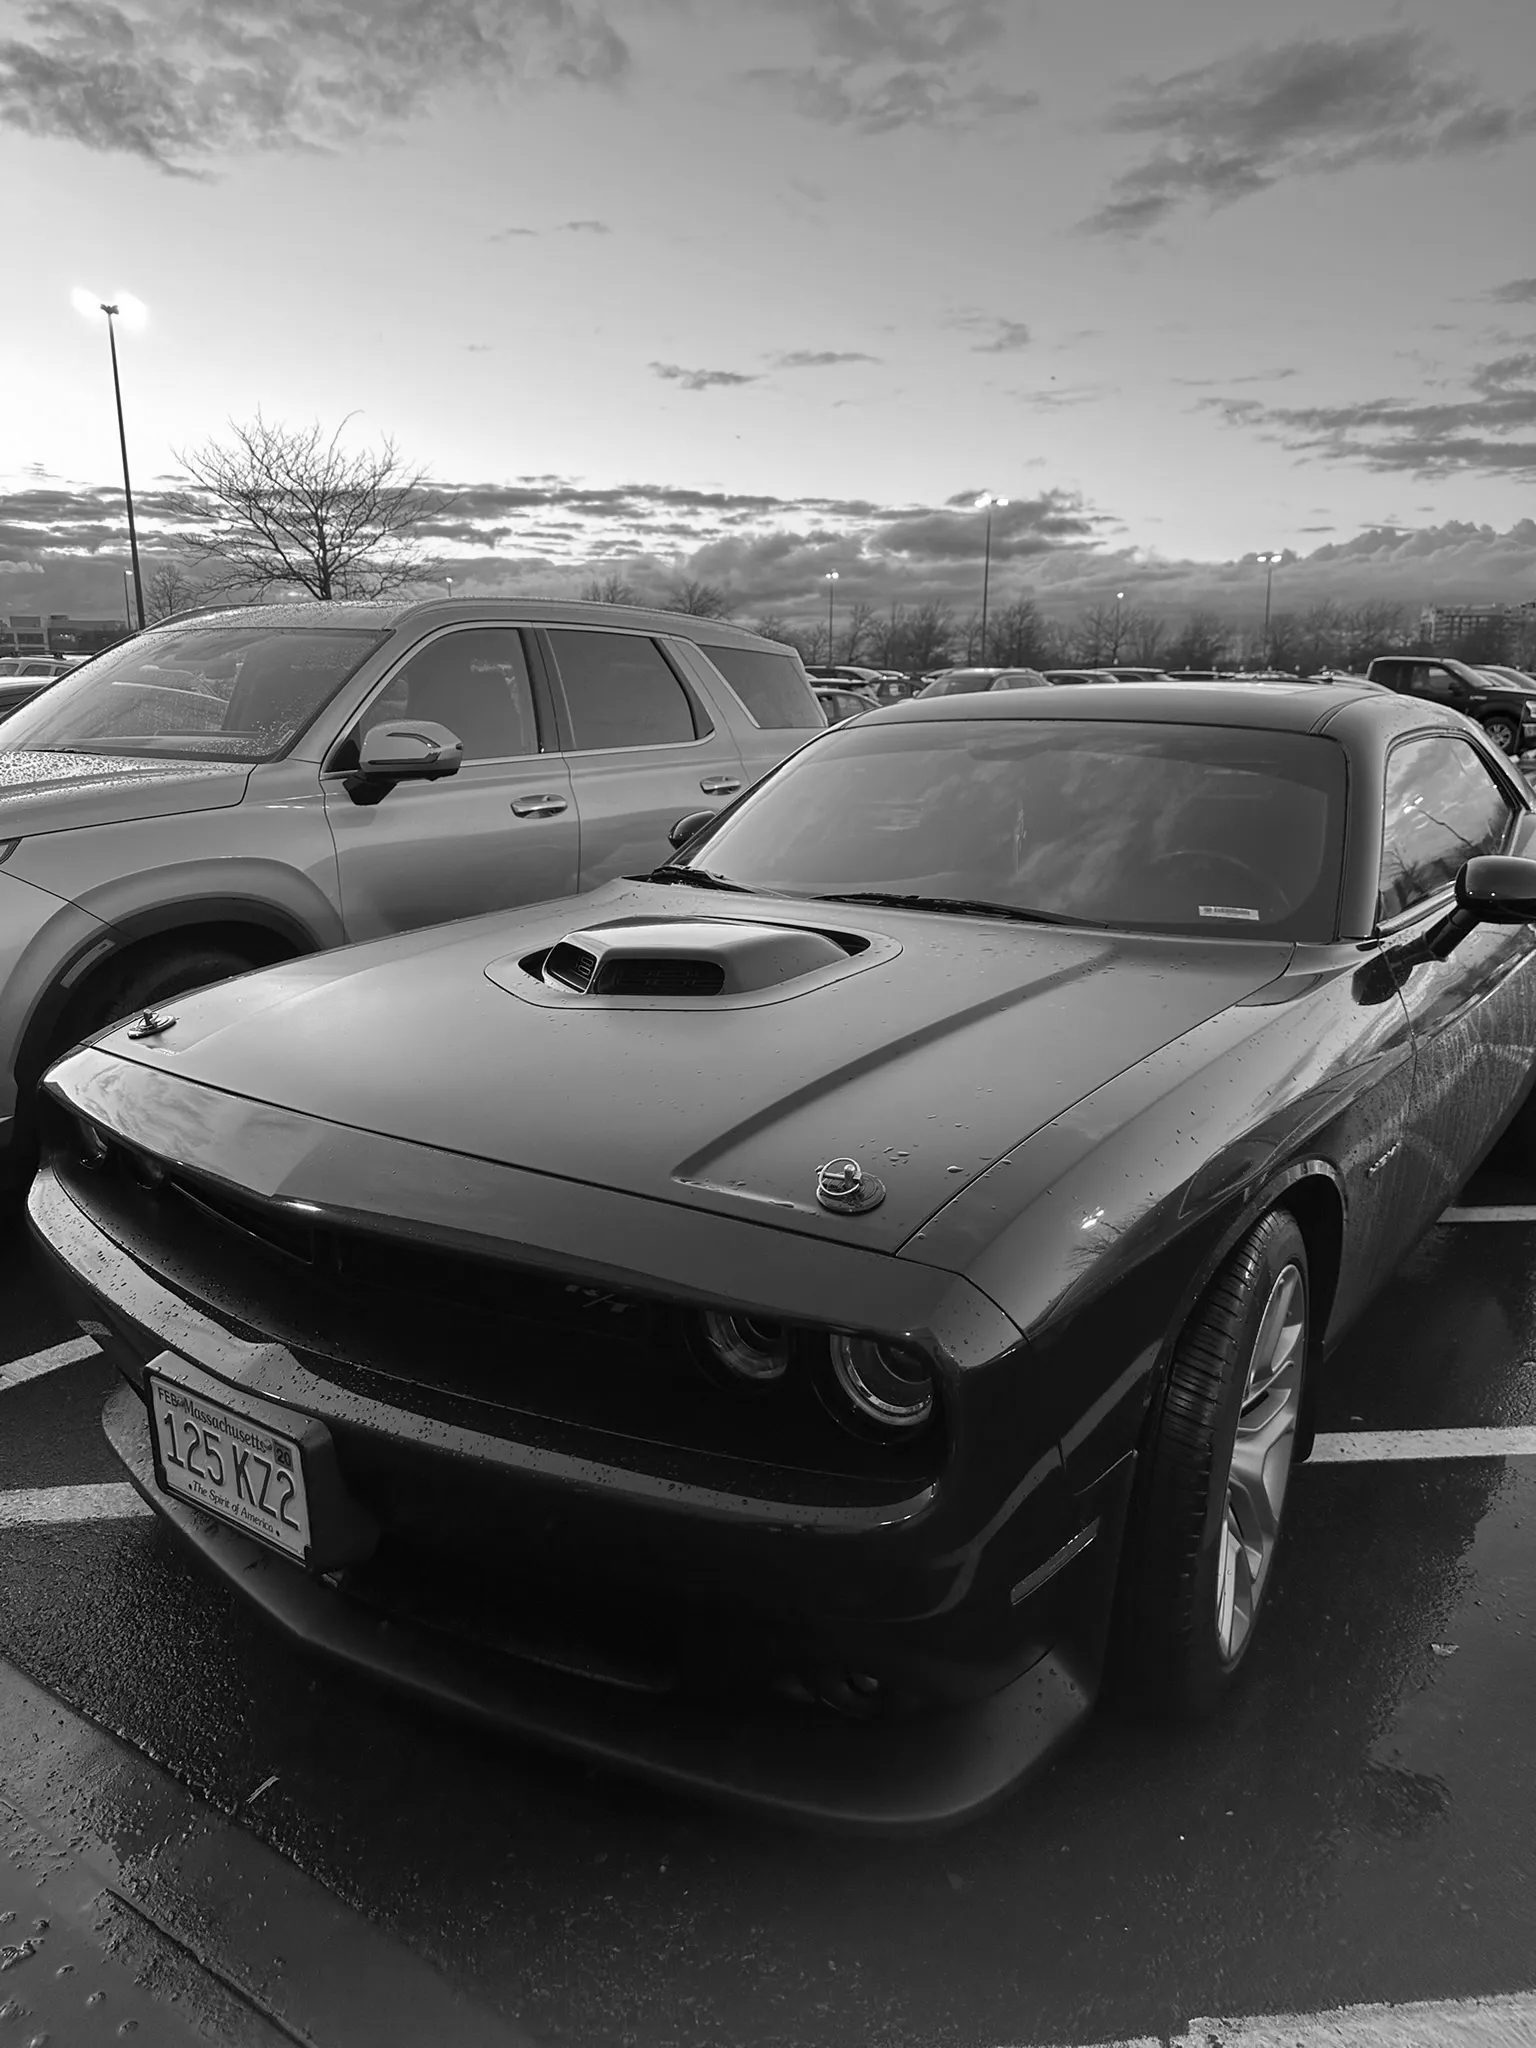
\includegraphics[width=0.9\textwidth]{car_2_grayscale.png}
        \caption{Car Grayscale}
        \label{fig:car_grayscale}
    \end{subfigure}
    \hfill
    \begin{subfigure}{0.4\textwidth}
        \centering
        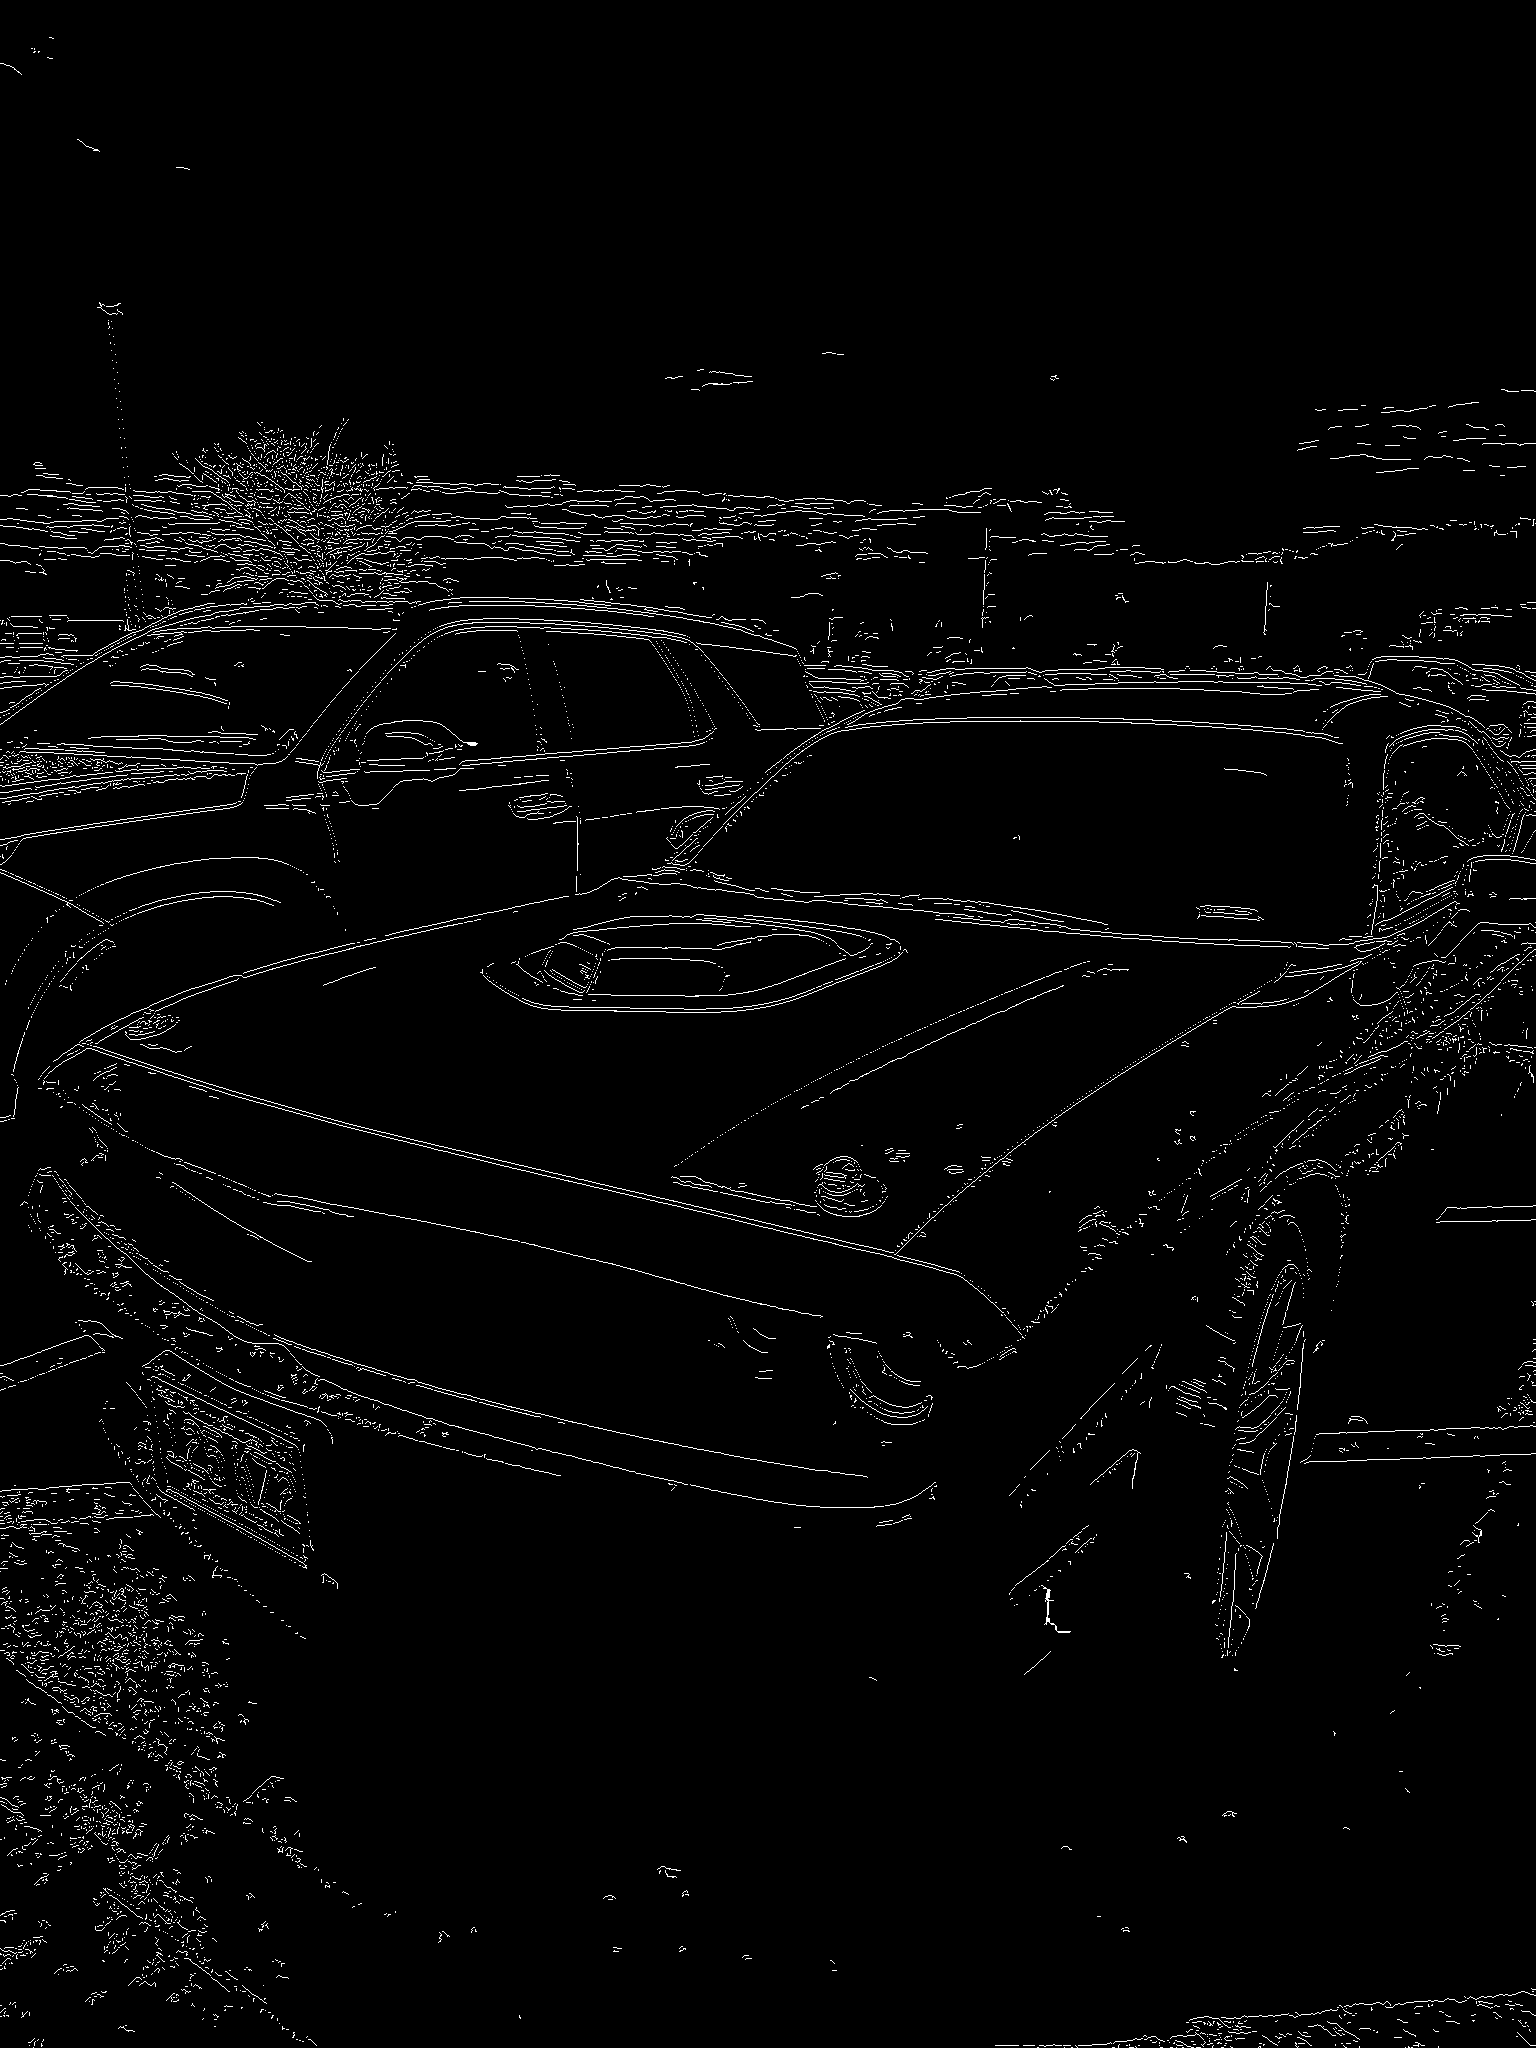
\includegraphics[width=0.9\textwidth]{car_8_canny_edge_detected.png}
        \caption{Car Edge Detected}
        \label{fig:car_edge_detected}
    \end{subfigure}
    \caption{Canny Edge Detection Results for Different Images (Part 5)}
\end{figure}

\clearpage

\subsection{Comparison of Different Thresholds}
The Canny Edge Detector was applied to the same image with different thresholds to observe the effect on edge detection. The results are shown in \autoref{fig:thresholds}.

\begin{figure}[ht]
    \centering
    \begin{subfigure}{0.3\textwidth}
        \centering
        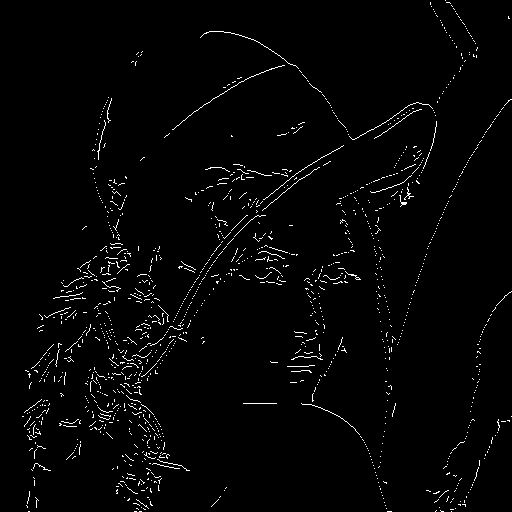
\includegraphics[width=0.9\textwidth]{lenna_8_canny_edge_detected0.01_0.2.png}
        \caption{Thresholds: 0.01, 0.2}
    \end{subfigure}
    \hfill
    \begin{subfigure}{0.3\textwidth}
        \centering
        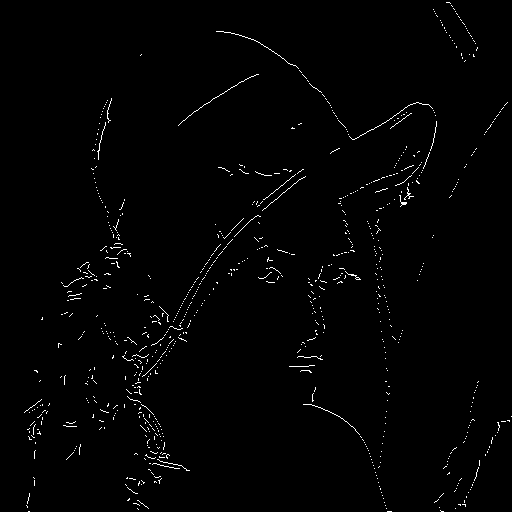
\includegraphics[width=0.9\textwidth]{lenna_8_canny_edge_detected0.01_0.3.png}
        \caption{Thresholds: 0.01, 0.3}
    \end{subfigure}
    \hfill
    \begin{subfigure}{0.3\textwidth}
        \centering
        
\includegraphics[width=0.9\textwidth]{lenna_8_canny_edge_detected0.1_0.15.png}
        \caption{Thresholds: 0.1, 0.15}
    \end{subfigure}
    
    \vspace{0.5cm}
    
    \begin{subfigure}{0.3\textwidth}
        \centering
        
\includegraphics[width=0.9\textwidth]{lenna_8_canny_edge_detected0.01_0.15.png}
        \caption{Thresholds: 0.01, 0.15}
    \end{subfigure}
    \hfill
    \begin{subfigure}{0.3\textwidth}
        \centering
        
\includegraphics[width=0.9\textwidth]{lenna_8_canny_edge_detected0.01_0.25.png}
        \caption{Thresholds: 0.01, 0.25}
    \end{subfigure}
    \hfill
    \begin{subfigure}{0.3\textwidth}
        \centering
        
\includegraphics[width=0.9\textwidth]{lenna_8_canny_edge_detected0.15_0.25.png}
        \caption{Thresholds: 0.15, 0.25}
    \end{subfigure}
    
    \caption{Canny Edge Detection Results with Different Thresholds}
    \label{fig:thresholds}
\end{figure}


% \clearpage

\section{Conclusion}
\label{sec:conclusion}

In this assignment, the Canny Edge Detection algorithm was implemented to identify edges in digital images effectively. The process involved applying Gaussian smoothing to reduce noise, calculating intensity gradients, and using non-maximum suppression to refine edge detection. Double thresholding and edge tracking by hysteresis were employed to produce the final edge map.

The results demonstrated the algorithm's ability to detect edges with high accuracy while minimizing noise and false detections. The findings highlight the importance of parameter tuning, such as the thresholds and Gaussian kernel size, in achieving optimal performance. Overall, the implementation validated the robustness and efficiency of the Canny Edge Detector in edge detection tasks.


\printbibliography[heading=bibintoc, title={References}]


% \section{Code Implementation}
\label{sec:code-implementation}

\end{document}
